\documentclass[12pt]{article}
\usepackage{amssymb}
\usepackage{amsmath}
\usepackage{tikz}
\usetikzlibrary{arrows, positioning}
\begin{document}
    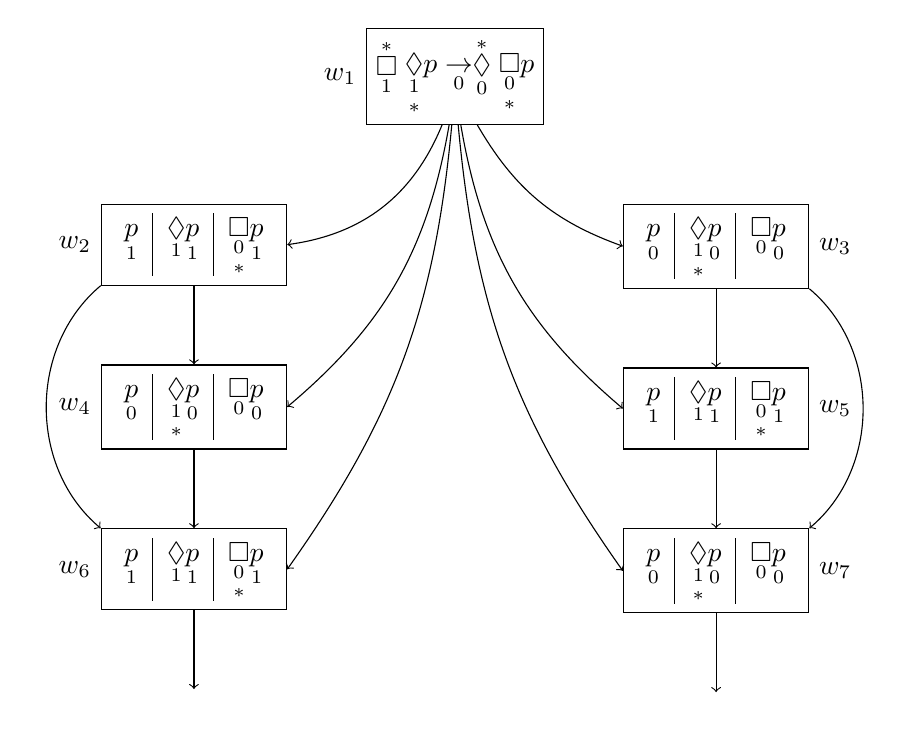
\begin{tikzpicture}[
    world/.style={rectangle,draw},
    invisible/.style={rectangle}]
        \node[world] (w_1)
              {$\underset{1}{\stackrel{*}{\Box}}
              \underset{*}{\underset{1}{\Diamond}} p
              \underset{0}{\rightarrow}
              \underset{0}{\stackrel{*}{\Diamond}}
              \underset{*}{\underset{0}{\Box}} p$};

        \node[black, left] at (w_1.west) {$w_1$};

        \node[world] (w_2) [below left=of w_1]
              {$\begin{array}{c|c|c}
                  \underset{1}{p} &
                \underset{1}{\Diamond}\underset{1}{p} &
                \underset{*}{\underset{0}{\Box}}\underset{1}{p}
              \end{array}$};

        \node[black, left] at (w_2.west) {$w_2$};

        \node[world] (w_3) [below right=of w_1]
              {$\begin{array}{c|c|c}
                  \underset{0}{p} &
                  \underset{*}{\underset{1}{\Diamond}}\underset{0}{p} &
                  \underset{0}{\Box}\underset{0}{p}
              \end{array}$};

        \node[black, right] at (w_3.east) {$w_3$};


        \node[world] (w_4) [below=of w_2]
            {$\begin{array}{c|c|c}
                \underset{0}{p} &
                \underset{*}{\underset{1}{\Diamond}} \underset{0}{p} &
                \underset{0}{\Box}\underset{0}{p}
            \end{array}$};

        \node[black, left] at (w_4.west) {$w_4$};


        \node[world] (w_5) [below=of w_3]
              {$\begin{array}{c|c|c}
                  \underset{1}{p} &
                \underset{1}{\Diamond}\underset{1}{p} &
                \underset{*}{\underset{0}{\Box}}\underset{1}{p}
              \end{array}$};

        \node[black, right] at (w_5.east) {$w_5$};


        \node[world] (w_6) [below=of w_4]
              {$\begin{array}{c|c|c}
                  \underset{1}{p} &
                \underset{1}{\Diamond}\underset{1}{p} &
                \underset{*}{\underset{0}{\Box}}\underset{1}{p}
              \end{array}$};

        \node[black, left] at (w_6.west) {$w_6$};


        \node[world] (w_7) [below=of w_5]
              {$\begin{array}{c|c|c}
                  \underset{0}{p} &
                  \underset{*}{\underset{1}{\Diamond}}\underset{0}{p} &
                  \underset{0}{\Box}\underset{0}{p}
              \end{array}$};

        \node[black, right] at (w_7.east) {$w_7$};


        \node[invisible] (i_1) [below=of w_6] {};
        \node[invisible] (i_2) [below=of w_7] {};

         \draw[->] (w_1) to[bend left = 30] (w_2.east);
         \draw[->] (w_1) to[bend right = 20] (w_3.west);

         \draw[->] (w_1) to[bend left = 20] (w_4.east);
         \draw[->] (w_2) -- (w_4);

         \draw[->] (w_1) to[bend right = 20] (w_5.west);
         \draw[->] (w_3) -- (w_5);

         \draw[->] (w_1) to[bend left = 15] (w_6.east);
         \draw[->] (w_2.south west) to[bend right = 50] (w_6.north west);
         \draw[->] (w_4) -- (w_6);

         \draw[->] (w_1) to[bend right = 15] (w_7.west);
         \draw[->] (w_3.south east) to[bend left = 50] (w_7.north east);
         \draw[->] (w_5) -- (w_7);

        \draw[->] (w_6) -- (i_1);
        \draw[->] (w_7) -- (i_2);

    \end{tikzpicture}
\end{document}
